\section{Cahier des charges du Projet "Barre-Franche"}
\subsection{Introduction technique}
Le projet qui nous est demandé est basé sur les SoC et plus particulièrement sur un FPGA, de chez Altera, embarqué dans un voilier pour en piloter la barre-franche.
\newline
Ce dispositif électronique fonctionnera à l'aide de différentes entrées/sorties (gyroscope, anémomètre, GPS, convertisseur analogique/numérique, vérin, boutons, buzzer).
\subsection{Cahier des charges général}
Durant ce projet, nous allons utiliser les différentes compétences acquises à travers les différents cours de l'année et les mettre en corrélation pour mener à bien ce dernier. Le projet devra respecter certains critères présentés ci-dessous :
\begin{enumerate}
    \item   Le dispositif devra utiliser un appareil de mesure pour capter la valeur de la vitesse du vent.
    \item   Le dispositif devra utiliser un appareil de mesure pour capter la direction du vent.
    \item   Le dispositif devra réceptionner des données GPS, traiter ces données et agir sur le dispositif en fonction des résultats obtenus après traitement.
    \item   Le dispositif devra avoir une interface entre l'opérateur et le voilier (boutons, Leds et buzzer).
    \item   Le dispositif devra piloter la barre-franche du voilier à l'aide des différents appareils pour venir piloter un vérin (Vérin et compas). 
\end{enumerate}\vspace{1cm}
La figure 1 modélise le système qui sera réalisé avec ses différentes fonctions et les différents flux d'informations nécessaires au système "Barre-Franche".
\begin{figure}[h]
  \begin{center}
    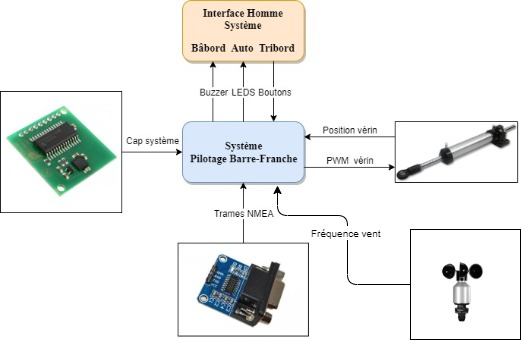
\includegraphics[width=0.8\textwidth]{images/Barre_franche.jpg}
    \caption{Diagramme contexte du système}
  \end{center}
\end{figure} 

\newpage 

Pour des raisons pratiques et de temps nous avons implémenté la mesure de la vitesse du vent, la gestion du vérin, la gestion du compas ainsi que l'asservissement du vérin, nous n'avons pas implémenté la gestion des trames NMEA, mais avons ajouté l'interface hommes système (boutons, leds et buzzer).

\subsection{Cahier des charges technique}
Le projet se porte sur la réalisation d'un dispositif embarqué à base de FPGA, de chez Altera. Il sera composé de deux parties principales une partie Hardware sur le FPGA et une partie Software intégrée/développée dans le FPGA (SOPC). Les deux parties communiqueront par le biais du Bus Avalon, qui est le Bus développé par Altera pour leur SOC.
Le cœur du projet sera composé d'un FPGA Cyclone IV EP4CE22F17C6N du fondeur Altera permettant le développement du projet Hardware et Software sur la même carte d'évaluation. Différentes fonctions seront implémentées :
\vspace{0.75cm}
\begin{enumerate}
    \item Une fonction qui permettra de lire la mesure de la vitesse du vent (0-250km/h). La fonction devra lire la sortie de l'anémomètre qui est une sortie logique de fréquence variable (0 à 250 Hz). 
    \item Une fonction générant un signal PWM qui sera utilisé dans plusieurs parties du projet. Cette fonction sera intégrée plus tard dans le SOPC du FPGA permettant la génération d'un signal PWM qu'on utilisera au travers du Bus Avalon.
    \item Une fonction de gestion vérin gérant le pilotage de la barre franche.
    \item Une fonction qui utilise un compas pour récupérer les mesures d'angles sur le plan horizontale du voilier, permettant de donner un cap à celui-ci.
    \item Une fonction qui permet la gestion de l'interface Homme système (composée de différents boutons[Bâbord, Tribord, Auto/Manuel], des LEDS ainsi qu'un buzzer).
    \item Une implémentation d'un MCU dans le FPGA grâce à l'outil SOPC du logiciel d'Altera. Celui-ci permettra le traitement et l'affichage des différentes variables du projet (cap du voilier, position vérin, position GPS, gestion des PWM et la vitesse du vent).
\end{enumerate}

\begin{figure}[h]
  \begin{center}
    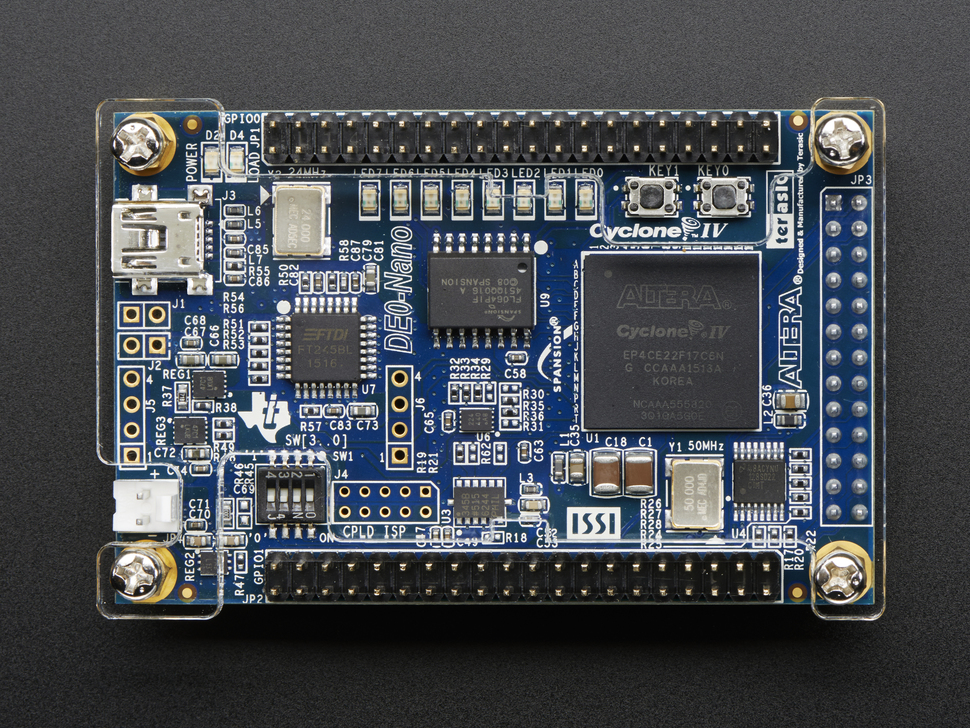
\includegraphics[width=0.5\textwidth]{images/DE0.jpg}
    \caption{DE0 Nano Altera}
  \end{center}
\end{figure}